% ============================================
%  Article Class (This is a LaTeX2e document)  
% ============================================
\documentclass[12pt]{scrartcl}

\usepackage[english]{babel}
\usepackage[utf8]{inputenc}

\usepackage{enumitem}
\usepackage[round]{natbib}
\usepackage{color}

\newcommand\reft[3][]{#2~\ref{#3}#1}
\newcommand\refp[3][]{(#2~\ref{#3}#1)}
\newcommand\refsect[1]{\reft{Section}{#1}}
\newcommand\refsecp[1]{\refp{Sec.}{#1}}
\newcommand\reftabt[1]{\reft{Table}{#1}}
\newcommand\reftabp[1]{\refp{Tab.}{#1}}

% ======
%  Math
% ======
\usepackage{amsmath}
\usepackage{amsthm}
\usepackage{mathtools} % \mathclap
\newtheorem{thm}{Theorem}[section]
\newtheorem{cor}[thm]{Corollary}
\newtheorem{lem}[thm]{Lemma}
\newtheorem{prop}[thm]{Proposition}
\newtheorem{property}[thm]{Property}
\theoremstyle{definition}
\newtheorem{defn}[thm]{Definition}
\newtheorem{assum}[thm]{Assumption}
\theoremstyle{remark}
\newtheorem{rem}[thm]{Remarque}
\numberwithin{equation}{section}
\newtheorem{req}[thm]{Requirement}

\usepackage{amssymb}
\newcommand{\prob}[1]{\mathbb{P}\left(#1\right)}
\newcommand{\Ker}[1]{\mathrm{Ker}\left(#1\right)}
\newcommand{\Image}[1]{\mathrm{Im}\left(#1\right)}
\newcommand{\diag}[1]{\mathrm{diag}\left(#1\right)}
\newcommand{\Vect}[1]{\mathrm{Vect}\left\{#1\right\}}

% ============================
%  Figures and relative paths
% ============================
\usepackage{graphicx}
\graphicspath{{figures/}}
\usepackage{import}
\makeatletter
  \def\relativepath{\import@path}
\makeatother
\newcommand\reffigt[2][]{\reft[#1]{Figure}{#2}}
\newcommand\reffigp[2][]{\refp[#1]{Fig.}{#2}}

% ==========
%  Document
% ==========
\begin{document}

\title{RBA pipeline}%
\author{S. Fischer - Biosys - MAIAGE}%
\date{\today}%

\maketitle

\newpage

\tableofcontents

\newpage

\section{Description of workflow}

\reffigt{fig:workflow} shows the global workflow of the pipeline. It contains four parts:
\begin{enumerate}
\item \textbf{PreRba}: Parsing of biological data into RBA compatible XML files. Parts of the process are semi-automated, meaning the user is needed to help solve ambiguous annotations.
\item \textbf{RbaXml}: Parsing/modifying XML files.
\item \textbf{RbaMatrices}: XML files are transformed into matrices.
\item \textbf{RbaSolver}: matrices are used to compute the optimal resource allocation.
\end{enumerate}
As a first step, this workflow should run for any prokaryote.

\begin{figure}[ht]
  \centering
  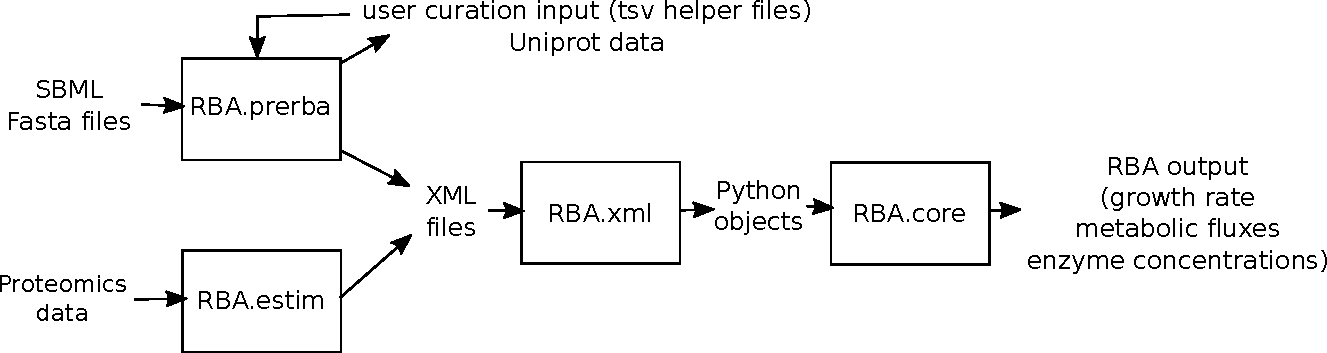
\includegraphics[width=\linewidth]{workflow}
  \caption{Workflow of pipeline. The lower part shows how compatibility between the workflow and the former version of RBA were maintained (used for consistency checks).}
  \label{fig:workflow}
\end{figure}

\subsection{Philosophy of the pipeline}

\paragraph{Everyting should work from first run on} We would like the pipeline to run completely on the first run. This means that a user that inputs an approximately standard SBML file should generate a full RBA model and get first growth rate results without having to do anything. Because annotations are often ambiguous, a lot of default parameters will be used for the first run, but the user will be able to parameterize their model progressively.

\paragraph{Helping user to setup main parameters through csv files} Conversion of biological data is very heavy and often ambiguous. When an annotation is ambiguous, the user will be asked for help through csv files. Everything that is input by the user is stored so the user does not have to provide the same information twice.

\paragraph{Helping user to setup fine parameters through xml files} After the main parameters have been set, the user will have ready-to-use RBA input files. We cannot handle every single parameter through csv files. Because RBA input files are written in xml, an advanced user will still be able to control more subtle parameters in a standardized (but programmatical) way.

\subsection{Typical expected usage}
\begin{enumerate}
\item The user provides SBML and runs the pipeline. They are happy because everything runs and he gets some output value. They are unhappy because this output value is unrealistic.
\item The user spends time going through the helper files and understands why they are here. They provide all the information needed to create a system fully adapted to their organism. They run the whole pipeline to see how growth rate has evolved and generate new and more consistent XML input files.
\item They spend time fine-tuning processes and enzyme catalytic efficiencies by modifying the XML files, finally reaching a biological sound model.
\end{enumerate}

\clearpage


\section{preRBA: converting biological data}

In order to get the workflow working, the user has to provide an SBML file describing the metabolism of their organism and a Uniprot file describing the proteins of their organism. This section lists the requirements that these files need to meet and how the user's help will be prompted while parsing them.

\subsection{SBML: extraction of metabolism and enzyme information}

\subsubsection{Requirements}
\req{File should contain \emph{only} metabolic reactions. User should remove the biomass reaction and reactions used to assemble non-metabolites (\textit{e.g.} proteins, rnas, etc.).}

\req{Every reaction should have a note containing a PROTEIN\_ASSOCIATION in standard form. This field should describe the composition of the enzymatic complex catalyzing the reaction in terms of proteins.}

\req{Name of proteins used in the PROTEIN\_ASSOCIATION field should correspond to the names listed in the \texttt{Gene names (ordered locus )} field of the uniprot file.}

\req{All proteins listed in the PROTEIN\_ASSOCIATION field should be referenced in the uniprot file.}

\subsubsection{User interactions}
Everything is automated, no help needed.

\subsection{Uniprot: extraction of protein information}

\subsubsection{Requirements}

\req{Uniprot file should be standard uniprot in TSV format.}

\subsubsection{User interactions}
\paragraph{Cofactor stoichiometry} Cofactor stoichiometry (and sometimes names) can be ambiguous. When necessary, user is prompted to read the \texttt{Cofactor} field and provide stoichiometry of cofactors. In order to limit interactions, note that we use the following rules to parse cofactor information:
\begin{itemize}
\item If field is empty, we assume there is no cofactor.
\item If we find exactly one name and its associated CHEBI identifier, and there is only one occurrence of the keyword \texttt{Binds}, we assume stoichiometry is the number the follows \texttt{Binds}.
\item If we find exactly one name and its associated CHEBI identifier, and there is no stoichiometry information using keyword \texttt{Binds}, we assume stoichiometry is 1.
\item In any other case, user is asked for help.
\end{itemize}

\paragraph{Subunit structure} Subunit structure is often ambiguous. When necessary, user is prompted to type how many copies of the proteins are usually found in the enzymatic complex. In order to limit interactions, note that we use the following rules to parse cofactor information:
\begin{itemize}
\item If field is empty, we assume there is one subunit in the complex.
\item If field contains exactly one occurence of the form ``\textit{prefix}mer'', we look at the prefix. If prefix is mono or heterodi, we assume stoichiomery is one. If prefix is homodi, homotri, homotera, homopenta, homohexa, hepta, homoocta, homodeca, homododeca, we assume the number of subunits corresponds to the prefix.
\item In any other case, user is asked for help.
\end{itemize}



\appendix


%\bibliographystyle{myplainnat}
%\bibliography{biblio}

\end{document}
% ----------------------------------------------------------------
